% ============================================================
%  INFORME TÉCNICO — Álgebra Lineal Aplicada
%  Péndulo invertido sobre un carro (dos configuraciones)
%  Universidad Nacional de Colombia — Sede Medellín · Facultad de Ciencias
%  Formato: artículo a una columna, estilo tesis/paper
% ============================================================
\documentclass[11pt,letterpaper]{article}

% ── Idioma y codificación ───────────────────────────────────
\usepackage[utf8]{inputenc}
\usepackage[T1]{fontenc}
\usepackage[spanish,provide=*]{babel}

% ── Tipografía (Palatino, look de tesis) ────────────────────
\usepackage{mathpazo}
\usepackage{microtype}
\linespread{1.02}

% ── Geometría de página ─────────────────────────────────────
\usepackage[letterpaper,top=0.9in,bottom=0.9in,left=1in,right=1in]{geometry}

% ── Matemáticas ─────────────────────────────────────────────
\usepackage{amsmath,amssymb,amsthm,mathtools,bm}

% ── Color, cajas, tablas, figuras ───────────────────────────
\usepackage{xcolor}
\definecolor{acento}{RGB}{31,59,107}
\definecolor{acento2}{RGB}{120,40,40}
\usepackage[most]{tcolorbox}
\usepackage{booktabs}
\usepackage{array}
\usepackage{graphicx}
\usepackage{tikz}
\usetikzlibrary{arrows.meta,calc,positioning}

% ── Títulos de sección ──────────────────────────────────────
\usepackage{titlesec}
\titleformat{\section}
  {\normalfont\large\bfseries\color{acento}}{\thesection}{0.7em}{}
\titleformat{\subsection}
  {\normalfont\normalsize\bfseries\color{acento!85!black}}{\thesubsection}{0.6em}{}
\titlespacing*{\section}{0pt}{1.1ex plus .8ex minus .2ex}{0.6ex plus .2ex}
\titlespacing*{\subsection}{0pt}{0.9ex plus .6ex minus .2ex}{0.45ex plus .2ex}

% ── Encabezado/pie ──────────────────────────────────────────
\usepackage{fancyhdr}
\pagestyle{fancy}\fancyhf{}
\renewcommand{\headrulewidth}{0.4pt}
\fancyhead[L]{\footnotesize\itshape Péndulo invertido sobre un carro}
\fancyhead[R]{\footnotesize\itshape Álgebra Lineal Aplicada}
\fancyfoot[C]{\thepage}

% ── Listas y enlaces ────────────────────────────────────────
\usepackage{enumitem}
\setlist{itemsep=2pt,topsep=3pt}
\usepackage[colorlinks=true,linkcolor=acento,citecolor=acento2,urlcolor=acento]{hyperref}
\usepackage{cleveref}

% ── Codigo fuente (listings) ────────────────────────────────
\usepackage{listings}
\definecolor{codecmt}{RGB}{110,120,130}
\definecolor{codekw}{RGB}{31,59,107}
\definecolor{codestr}{RGB}{120,40,40}
\lstdefinestyle{julia}{%
  basicstyle=\ttfamily\scriptsize,
  keywordstyle=\color{codekw}\bfseries,
  commentstyle=\color{codecmt}\itshape,
  stringstyle=\color{codestr},
  showstringspaces=false,
  breaklines=true,
  columns=fullflexible,
  frame=single,
  rulecolor=\color{acento!45!black},
  framesep=4pt,
  xleftmargin=6pt,xrightmargin=6pt,
  aboveskip=6pt,belowskip=6pt,
  morekeywords={function,end,for,while,if,else,elseif,return,using,import,module,struct,begin,in}
}
\lstset{style=julia}

% ── Ruta de figuras generadas ───────────────────────────────
\graphicspath{{figs/}}

% ── Teoremas ────────────────────────────────────────────────
\theoremstyle{definition}
\newtheorem{definicion}{Definición}[section]
\newtheorem{ejemplo}[definicion]{Ejemplo}
\theoremstyle{plain}
\newtheorem{teorema}[definicion]{Teorema}
\newtheorem{proposicion}[definicion]{Proposición}
\newtheorem{lema}[definicion]{Lema}
\newtheorem{corolario}[definicion]{Corolario}
\theoremstyle{remark}
\newtheorem{observacion}[definicion]{Observación}
\newtheorem{hipotesis}[definicion]{Hipótesis}
\renewcommand{\qedsymbol}{$\blacksquare$}

% ── Caja para resultados clave ──────────────────────────────
\newtcolorbox{clave}[1][]{colback=acento!4,colframe=acento!55!black,
  boxrule=0.6pt,arc=2pt,left=6pt,right=6pt,top=5pt,bottom=5pt,#1}

% ── Operadores ──────────────────────────────────────────────
\DeclareMathOperator{\rank}{rango}
\DeclareMathOperator{\Imo}{Im}
\DeclareMathOperator{\nuc}{N}
\DeclareMathOperator{\gen}{gen}
\DeclareMathOperator{\Real}{Re}
\newcommand{\R}{\mathbb{R}}
\newcommand{\C}{\mathbb{C}}
\newcommand{\TM}{\mathrm{T}M}
\newcommand{\calC}{\mathcal{C}}
\newcommand{\calO}{\mathcal{O}}
\newcommand{\xv}{\bm{x}}
\newcommand{\uv}{\bm{u}}
\newcommand{\yv}{\bm{y}}
\newcommand{\rv}{\bm{r}}

% ── cleveref en español ─────────────────────────────────────
\crefname{equation}{ec.}{ecs.}\Crefname{equation}{Ecuación}{Ecuaciones}
\crefname{section}{sección}{secciones}\Crefname{section}{Sección}{Secciones}
\crefname{figure}{figura}{figuras}\Crefname{figure}{Figura}{Figuras}
\crefname{table}{tabla}{tablas}\Crefname{table}{Tabla}{Tablas}
\crefname{definicion}{definición}{definiciones}\Crefname{definicion}{Definición}{Definiciones}
\crefname{teorema}{teorema}{teoremas}\Crefname{teorema}{Teorema}{Teoremas}
\crefname{proposicion}{proposición}{proposiciones}\Crefname{proposicion}{Proposición}{Proposiciones}
\crefname{corolario}{corolario}{corolarios}\Crefname{corolario}{Corolario}{Corolarios}
\crefname{observacion}{observación}{observaciones}\Crefname{observacion}{Observación}{Observaciones}
\crefname{hipotesis}{hipótesis}{hipótesis}\Crefname{hipotesis}{Hipótesis}{Hipótesis}
\crefname{appendix}{apéndice}{apéndices}\Crefname{appendix}{Apéndice}{Apéndices}
\AtBeginDocument{%
  \renewcommand{\crefpairconjunction}{ y }%
  \renewcommand{\creflastconjunction}{ y }%
  \renewcommand{\crefmiddleconjunction}{, }%
}
\addto\captionsspanish{\renewcommand{\tablename}{Tabla}}

% ============================================================
\begin{document}

% ── Portada ─────────────────────────────────────────────────
\begin{center}
    {\footnotesize\bfseries\color{acento2} INFORME TÉCNICO}\\[0.4em]
    {\LARGE\bfseries Análisis del Péndulo Invertido sobre un Carro \\[0.2em] mediante Álgebra Lineal Aplicada}\\[0.5em]
    {\large Espacio de Estados, Análisis Espectral y Control por \\ Realimentación de Estado en Dos Configuraciones}\\[1.2em]
    {\normalsize Mateo Bedoya Rojas \quad\textbullet\quad Santiago Uribe Echavarría \quad\textbullet\quad Camilo Alejandro Patiño Osorio}\\[0.5em]
    {\footnotesize
    Facultad de Ciencias, Universidad Nacional de Colombia, Sede Medellín \\ \texttt{mabedoyar@unal.edu.co} \quad \texttt{sauribee@unal.edu.co} \quad \texttt{cpatinoo@unal.edu.co}}\\[0.8em]
\end{center}
\vspace{0.4em}
\hrule height 0.6pt
\vspace{1.0em}

% ── Resumen ─────────────────────────────────────────────────
\begin{abstract}
\noindent
Se presenta un estudio, formulado en el lenguaje del cálculo variacional, resuelto por 
métodos matriciales y herramientas de álgebra lineal, de dos configuraciones 
del sistema clásico \emph{péndulo invertido sobre un carro}: el 
péndulo \emph{simple} (una barra articulada al carro) y el
péndulo \emph{doble} (dos eslabones en serie, con la masa principal en el
extremo superior). Para cada configuración se deducen, paso a paso, las
ecuaciones de movimiento mediante el formalismo de Euler--Lagrange; se
precisa el marco geométrico del problema --- coordenadas generalizadas,
espacio de configuración, espacio de estados y espacio de caminos --- y
se linealiza el sistema alrededor del equilibrio vertical inestable
mediante una aproximación de Taylor de primer orden, obteniendo una
representación en espacio de estados $\dot\xv=A\xv+B\uv$. Sobre esta
representación se despliegan las herramientas centrales: la exponencial
matricial como operador solución, el análisis espectral y el teorema de 
Cayley--Hamilton, el polinomio minimal y las descomposiciones canónicas (Jordan), 
la estabilidad en el sentido de Hurwitz y de Lyapunov, y los criterios de 
rango de Kalman para controlabilidad y observabilidad. Con ellas se diseñan controladores por
realimentación de estado $\uv=-K\xv$, por asignación de polos (fórmula de
Ackermann) y por regulación lineal cuadrática (LQR, vía la ecuación
algebraica de Riccati), verificados numéricamente. El informe muestra
cómo un puñado de conceptos del álgebra lineal constituye el lenguaje
natural para modelar, analizar y controlar un sistema dinámico.
\end{abstract}

\vspace{0.3em}
\noindent\textbf{Palabras clave:}\;
péndulo invertido, péndulo doble, espacio de estados, exponencial
matricial, eigenvalores, controlabilidad, observabilidad, asignación de
polos, LQR, álgebra lineal.
\vspace{0.8em}
\hrule height 0.4pt
\vspace{1.0em}

% ============================================================
\section{El problema}
\label{sec:problema}

El \emph{péndulo invertido sobre un carro} es uno de los problemas más
estudiados de la teoría de control y de los sistemas dinámicos
\cite{ogata2010,chen1999}. El montaje es sencillo de describir: un carro
se desplaza sobre un riel horizontal y sobre él se articula un péndulo.
La posición de interés es la \emph{vertical superior}, en la que el
péndulo apunta hacia arriba. Esa posición es un equilibrio, pero un
equilibrio \emph{inestable}: la más mínima perturbación hace que el
péndulo se aleje y caiga. El objetivo de control es aplicar una fuerza
horizontal $u(t)$  únicamente sobre el carro que 
mantenga el péndulo erguido pese a esa tendencia a caer por la gravedad.

Existen tres aspectos que hacen interesante el estudio:
\emph{subactuado}: hay más grados de libertad que actuadores, pues con la
única fuerza sobre el carro debemos gobernar a la vez la posición del
carro y el ángulo del péndulo. Es \emph{inestable} en lazo abierto, de
modo que sin control no se sostiene. Y su dinámica es \emph{no lineal},
por la presencia de funciones trigonométricas del ángulo. Estos tres
rasgos --- subactuación, inestabilidad y no linealidad --- son los que
aparecen, a mayor escala, en problemas reales como la estabilización de
cohetes, la marcha de robots bípedos o el equilibrio de vehículos de dos
ruedas.

Su interés para el estudio y resolución mediante herramientas de álgebra lineal aplicada es que casi todas las
preguntas que se derivan  sobre el sistema se responden con álgebra
lineal. ¿Cómo evolucionan las pequeñas desviaciones del equilibrio? Lo
dice la \emph{exponencial de una matriz}. ¿Es estable o inestable? Lo
deciden los \emph{eigenvalores} de esa matriz. ¿Podemos, con la fuerza
del carro, influir en todos los modos del sistema? Es una pregunta de
\emph{rango}. ¿Podemos reconstruir el estado completo a partir de unas
pocas mediciones? También es de rango. Y diseñar el control consiste en
\emph{reubicar los eigenvalores} de una matriz mediante realimentación y utilizar los métodos para diseñar un controlador.

Este informe analiza dos versiones del
sistema, donde una se obtiene de la primera, aumentando la complejidad:

\begin{itemize}
  \item \textbf{Configuración I --- péndulo simple.} Una barra rígida
  uniforme articulada al carro (\cref{fig:simple}). Tiene dos grados de
  libertad, su estado vive en $\R^4$ y posee un único modo inestable.
  \item \textbf{Configuración II --- péndulo doble.} Se añade un segundo
  eslabón, de modo que aparecen dos masas en serie y la masa superior
  queda en el extremo (\cref{fig:doble}). Tiene tres grados de libertad,
  su estado vive en $\R^6$ y posee \emph{dos} modos inestables.
\end{itemize}


La segunda configuración es deliberadamente más exigente: muestra que el
mismo razonamiento algebraico --- linealizar, estudiar el espectro,
verificar controlabilidad, diseñar la realimentación --- escala sin
cambios conceptuales cuando crecen los grados de libertad, solo a costa
de matrices más grandes y mayor esfuerzo de control.

\paragraph{Estructura del informe.} Siguiendo el esquema de un informe
técnico, la \cref{sec:formal} \emph{formaliza} el problema: fija el marco
geométrico, deduce los lagrangianos y las ecuaciones de movimiento de
ambas configuraciones, las lineariza y las lleva al espacio de estados.
La \cref{sec:herr} reúne y justifica las \emph{herramientas} de álgebra
lineal. La \cref{sec:metodo} describe la \emph{metodología} de cómputo y
cómo se obtuvo cada resultado. La \cref{sec:result} presenta los
\emph{resultados} numéricos, y la \cref{sec:concl} concluye. Los
apéndices contienen las derivaciones algebraicas y la verificación
numérica.

% ============================================================
\section{Formalización del problema}
\label{sec:formal}

\subsection{Coordenadas generalizadas y espacios del problema}
\label{sub:espacios}

Antes de escribir una sola ecuación conviene precisar qué objetos
intervienen y en qué conjunto vive cada uno. El lenguaje es el de la
mecánica lagrangiana, tal como se introduce en las notas del curso
\cite{notas2026}, y se apoya en la teoría de sistemas dinámicos
\cite{hirsch2004}.

\paragraph{Coordenadas generalizadas.} Un sistema mecánico puede
describirse con muchas coordenadas, pero la mayoría están ligadas por
restricciones (las barras son rígidas, el carro no se levanta del riel).
Las \emph{coordenadas generalizadas} $q=(q_1,\dots,q_d)$ son un conjunto
\emph{mínimo} de números independientes que determinan por completo la
configuración una vez impuestas todas las restricciones. El entero $d$ es
el número de \emph{grados de libertad}. Se eligen de manera que sean consistentes con la formulación, pues así se incorporan las restricciones \emph{desde el
comienzo} en lugar de arrastrarlas como ecuaciones adicionales.

Para el péndulo simple bastan dos números: la posición horizontal del
carro $x$ y el ángulo $\theta$ del péndulo, de modo que $q=(x,\theta)$ y
$d=2$. Para el péndulo doble se requiere un ángulo por eslabón,
$q=(x,\theta_1,\theta_2)$, y $d=3$.

\begin{definicion}[Espacio de configuración]
\label{def:config}
El \emph{espacio de configuración} $M$ es el conjunto de todas las
configuraciones admisibles del sistema, parametrizado por las coordenadas
generalizadas. Es una variedad diferenciable de dimensión $d$.
\end{definicion}

$M$ tiene esta forma pues la posición del carro es un número
real cualquiera, así que aporta un factor $\R$. El ángulo, en cambio, no es un número real cualquiera: $\theta$ y $\theta+2\pi$ representan la
\emph{misma} configuración física, de modo que el ángulo vive en la
circunferencia $S^1$ y no en $\R$. Por eso, para el péndulo simple,
$M=\R\times S^1$, y para el doble, $M=\R\times S^1\times S^1$. Como aquí
solo interesa una vecindad del equilibrio (ángulos pequeños), podemos
identificar localmente $S^1$ con $\R$ y tratar $M$ como $\R^2$ o $\R^3$;
pero es importante saber de dónde viene esa identificación.

La configuración no basta pues las leyes de la mecánica
(Newton, y de forma equivalente la formulación de Euler--Lagrange) son ecuaciones
diferenciales de \emph{segundo orden} en el tiempo. Para predecir el
futuro de una ecuación de segundo orden no alcanza con la posición: hace
falta también la \emph{velocidad} inicial. Dos configuraciones iguales
con velocidades distintas tienen futuros distintos. Por eso el objeto que
determina la evolución no es $q$, sino el par $(q,\dot q)$.

\begin{definicion}[Espacio de estados]
\label{def:estados}
El \emph{espacio de estados} es el \emph{fibrado tangente} $\TM$, cuyos
puntos son los pares posición--velocidad
$(q,\dot q)=(q_1,\dots,q_d,\dot q_1,\dots,\dot q_d)$, de dimensión $2d$.
Para cada $q\in M$, las velocidades admisibles forman el \emph{espacio
tangente} $\mathrm{T}_qM$; la unión de todos ellos es $\TM$.
\end{definicion}

Conocer un punto de $\TM$ equivale a conocer el
estado completo, y el teorema de existencia y unicidad para ecuaciones
diferenciales garantiza que ese estado determina una única trayectoria
futura. Así, el estado del péndulo simple vive en $\R^4$ y el del doble
en $\R^6$.

\begin{definicion}[Lagrangiano]
\label{def:lagrangiano}
El \emph{lagrangiano} es la función
\begin{equation}\label{eq:Ldef}
  L:\TM\longrightarrow\R,\qquad L(q,\dot q)=T(q,\dot q)-V(q),
\end{equation}
donde $T$ es la energía cinética (depende de posiciones y velocidades) y
$V$ la energía potencial (depende solo de posiciones).
\end{definicion}

El lagrangiano \emph{parte} de un estado
$(q,\dot q)\in\TM$ y \emph{devuelve} un número real. No es una fuerza ni
una trayectoria: es una densidad escalar que, integrada en el tiempo,
mide el ``costo'' de una trayectoria. La elección $L=T-V$ no es
arbitraria; proviene del principio variacional siguiente.

\begin{definicion}[Espacio de caminos y acción]
\label{def:caminos}
Fijados un intervalo $[t_1,t_2]$ y dos configuraciones $q_a,q_b\in M$, el
\emph{espacio de caminos} es el conjunto de trayectorias suaves con esos
extremos,
\begin{equation}
  \mathcal{P}=\{\,\gamma\in C^{\infty}([t_1,t_2],M):
                \gamma(t_1)=q_a,\ \gamma(t_2)=q_b\,\}.
\end{equation}
Sobre él se define el \emph{funcional de acción}
\begin{equation}\label{eq:accion}
  S:\mathcal{P}\longrightarrow\R,\qquad
  S[\gamma]=\int_{t_1}^{t_2} L\bigl(\gamma(t),\dot\gamma(t)\bigr)\,dt.
\end{equation}
\end{definicion}

El espacio de caminos $\mathcal{P}$ es de dimensión infinita: cada uno de
sus ``puntos'' es una trayectoria completa. El funcional $S$ asigna a
cada trayectoria un número (su acción). El principio de Hamilton afirma
que las trayectorias \emph{físicas} hacen estacionaria la acción
($\delta S=0$): son los puntos críticos de $S$. Es el análogo, en
dimensión infinita, de buscar dónde se anula la derivada de una función.

\subsection{El lagrangiano y las ecuaciones de Euler--Lagrange}
\label{sub:euler}

Imponer $\delta S=0$ sobre \cref{eq:accion} conduce a un sistema de
ecuaciones diferenciales que son las ecuaciones de movimiento.

\begin{teorema}[Ecuaciones de Euler--Lagrange]
\label{thm:EL}
Una trayectoria $\gamma$ es un punto crítico de la acción
\cref{eq:accion} si y solo si satisface, para cada coordenada
$i=1,\dots,d$,
\begin{equation}\label{eq:EL}
  \frac{d}{dt}\!\left(\frac{\partial L}{\partial \dot q_i}\right)
  -\frac{\partial L}{\partial q_i}=Q_i,
\end{equation}
donde $Q_i$ es la fuerza generalizada \emph{no conservativa} asociada a
$q_i$ (en nuestro caso, la fuerza de control y la fricción).
\end{teorema}

\begin{observacion}
Cuando todas las fuerzas derivan de un potencial, $Q_i=0$ y se recupera
la forma usual de Euler--Lagrange. El término $Q_i$ es la vía estándar
para incorporar fuerzas externas (el control $u$) y disipativas (la
fricción $-b\dot x$) que no provienen de $V$.
\end{observacion}

El plan de trabajo queda fijado y es el mismo para las dos
configuraciones: (i) elegir las coordenadas; (ii) escribir las posiciones
de cada masa y derivarlas para obtener las velocidades; (iii) formar $T$
y $V$, y con ellas $L=T-V$; (iv) aplicar \cref{eq:EL} para obtener las
ecuaciones no lineales; (v) linealizar y reescribir el resultado en el
espacio de estados.

\subsection{Configuración I: péndulo simple sobre el carro}
\label{sub:simple}

\begin{figure}[htbp]
  \centering
  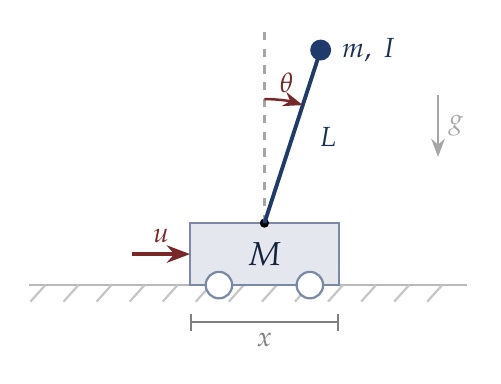
\begin{tikzpicture}[>=Stealth,thick,scale=1.05]
    \draw[gray!55] (-1.7,0) -- (3.6,0);
    \foreach \i in {-1.5,-1.1,...,3.4}{\draw[gray!45] (\i,0)--(\i-0.18,-0.2);}
    \draw[fill=acento!12,draw=acento!60] (0.25,0) rectangle (2.05,0.75);
    \node[acento!60!black] at (1.15,0.375) {\large $M$};
    \draw[fill=white,draw=acento!60] (0.6,0) circle (0.16);
    \draw[fill=white,draw=acento!60] (1.7,0) circle (0.16);
    \coordinate (P) at (1.15,0.75);
    \fill (P) circle (1.6pt);
    \coordinate (B) at ($(P)+(72:2.2)$);
    \draw[dashed,gray!70] (P) -- ++(0,2.35);
    \draw[acento,line width=1.4pt] (P) -- (B);
    \fill[acento] (B) circle (3.6pt);
    \node[right=4pt,acento!80!black] at (B) {$m,\ I$};
    \draw[->,acento2,line width=0.9pt] (P)++(0,1.5) arc(90:72:1.5);
    \node[acento2] at ($(P)+(81:1.72)$) {$\theta$};
    \node[right=6pt,acento!80!black] at ($(P)!0.5!(B)$) {$L$};
    \draw[->,line width=1.2pt,acento2] (-0.45,0.375)--(0.25,0.375) node[midway,above]{$u$};
    \draw[|-|,gray] (0.25,-0.45)--(2.05,-0.45) node[midway,below]{$x$};
    \draw[->,gray!70] (3.25,2.3)--(3.25,1.55) node[midway,right]{$g$};
  \end{tikzpicture}
  \caption{Configuración I. Péndulo invertido simple sobre el carro. La
  barra uniforme tiene masa $m$, longitud total $2L$ (distancia del
  pivote al centro de masa $L$) y momento de inercia $I$ respecto a su
  centro de masa. El ángulo $\theta$ se mide desde la vertical
  \emph{superior}: $\theta=0$ es el equilibrio erguido.}
  \label{fig:simple}
\end{figure}

\textbf{Coordenadas y posiciones.} Tomamos $q=(x,\theta)$, con $\theta$
medido desde la vertical superior. El centro de masa del carro está en
$(x,0)$ con velocidad $(\dot x,0)$. El centro de masa de la barra se halla
a distancia $L$ del pivote a lo largo de ella; con $\theta$ medido desde
la vertical,
\begin{equation}\label{eq:rcm-simple}
  \rv_{\mathrm{cm}}=(x+L\sin\theta,\ L\cos\theta).
\end{equation}

\textbf{Velocidades.} Derivando \cref{eq:rcm-simple} respecto del tiempo
(regla de la cadena, con $\theta=\theta(t)$),
\begin{equation}\label{eq:vcm-simple}
  \dot\rv_{\mathrm{cm}}=(\dot x+L\dot\theta\cos\theta,\ -L\dot\theta\sin\theta),
\end{equation}
cuyo módulo al cuadrado, usando $\cos^2\theta+\sin^2\theta=1$, es
\begin{align}
  \lVert\dot\rv_{\mathrm{cm}}\rVert^2
  &=(\dot x+L\dot\theta\cos\theta)^2+(L\dot\theta\sin\theta)^2 \notag\\
  &=\dot x^2+2L\dot x\dot\theta\cos\theta+L^2\dot\theta^2.
  \label{eq:speed2-simple}
\end{align}

\textbf{Energías y lagrangiano.} La energía cinética suma la traslación
del carro, la traslación del centro de masa de la barra y la rotación de
la barra ($\tfrac12 I\dot\theta^2$):
\begin{equation}\label{eq:T-simple}
  T=\tfrac12 M\dot x^2
   +\tfrac12 m\bigl(\dot x^2+2L\dot x\dot\theta\cos\theta+L^2\dot\theta^2\bigr)
   +\tfrac12 I\dot\theta^2.
\end{equation}
La energía potencial, con referencia en la altura del pivote, es
\begin{equation}\label{eq:V-simple}
  V=mgL\cos\theta,
\end{equation}
y el lagrangiano es $L=T-V$.

\textbf{Ecuaciones de movimiento.} Aplicando \cref{eq:EL} a $q_1=x$ con
$Q_1=u-b\dot x$ y a $q_2=\theta$ con $Q_2=0$ se obtiene el sistema no
lineal (detalle en el \cref{anx:lag})
\begin{subequations}\label{eq:nl-simple}
\begin{align}
  (M{+}m)\ddot x+mL\ddot\theta\cos\theta
    -mL\dot\theta^2\sin\theta+b\dot x &= u,\\
  (I{+}mL^2)\ddot\theta+mL\ddot x\cos\theta
    -mgL\sin\theta &= 0.
\end{align}
\end{subequations}

\begin{observacion}[La firma de la inestabilidad]
\label{obs:firma}
El término $-mgL\sin\theta$ es el que vuelve inestable el equilibrio
superior: al linealizar produce un coeficiente \emph{positivo} que
originará un eigenvalor real positivo. Si el péndulo colgara hacia abajo,
ese término aparecería con signo opuesto y el equilibrio sería estable.
La diferencia entre ``colgar'' y ``estar invertido'' es, literalmente, un
signo.
\end{observacion}

\subsection{Configuración II: péndulo doble sobre el carro}
\label{sub:doble}

\begin{figure}[htbp]
  \centering
  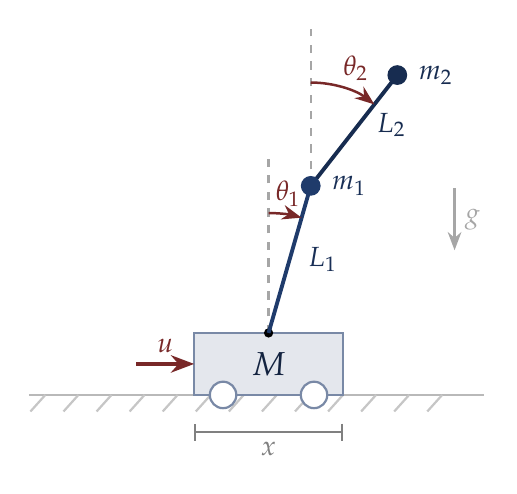
\begin{tikzpicture}[>=Stealth,thick,scale=1.05]
    \draw[gray!55] (-1.5,0) -- (4.0,0);
    \foreach \i in {-1.3,-0.9,...,3.8}{\draw[gray!45] (\i,0)--(\i-0.18,-0.2);}
    \draw[fill=acento!12,draw=acento!60] (0.5,0) rectangle (2.3,0.75);
    \node[acento!60!black] at (1.4,0.375) {\large $M$};
    \draw[fill=white,draw=acento!60] (0.85,0) circle (0.16);
    \draw[fill=white,draw=acento!60] (1.95,0) circle (0.16);
    \coordinate (P0) at (1.4,0.75);
    \coordinate (P1) at ($(P0)+(74:1.85)$);
    \coordinate (P2) at ($(P1)+(52:1.7)$);
    \draw[dashed,gray!70] (P0) -- ++(0,2.2);
    \draw[dashed,gray!70] (P1) -- ++(0,1.9);
    \fill (P0) circle (1.6pt);
    \draw[acento,line width=1.4pt] (P0) -- (P1);
    \draw[acento!75!black,line width=1.4pt] (P1) -- (P2);
    \fill[acento] (P1) circle (3.4pt);
    \fill[acento!75!black] (P2) circle (3.4pt);
    \node[right=4pt,acento!80!black] at (P1) {$m_1$};
    \node[right=4pt,acento!75!black] at (P2) {$m_2$};
    \draw[->,acento2,line width=0.9pt] (P0)++(0,1.45) arc(90:74:1.45);
    \node[acento2] at ($(P0)+(82:1.7)$) {$\theta_1$};
    \draw[->,acento2,line width=0.9pt] (P1)++(0,1.25) arc(90:52:1.25);
    \node[acento2] at ($(P1)+(69:1.52)$) {$\theta_2$};
    \node[right=3pt,acento!80!black] at ($(P0)!0.5!(P1)$) {$L_1$};
    \node[right=3pt,acento!75!black] at ($(P1)!0.55!(P2)$) {$L_2$};
    \draw[->,line width=1.2pt,acento2] (-0.2,0.375)--(0.5,0.375) node[midway,above]{$u$};
    \draw[|-|,gray] (0.5,-0.45)--(2.3,-0.45) node[midway,below]{$x$};
    \draw[->,gray!70] (3.65,2.5)--(3.65,1.75) node[midway,right]{$g$};
  \end{tikzpicture}
  \caption{Configuración II. Péndulo invertido doble sobre el carro.
  Eslabones de longitudes $L_1$ (inferior) y $L_2$ (superior), con masas
  puntuales $m_1$ en la articulación intermedia y $m_2$ en el extremo
  superior. Cada ángulo $\theta_1,\theta_2$ se mide desde \emph{su propia}
  vertical (líneas discontinuas), convención que produce las matrices
  linealizadas más limpias.}
  \label{fig:doble}
\end{figure}

\textbf{Coordenadas y posiciones.} Tomamos $q=(x,\theta_1,\theta_2)$, con
masas puntuales $m_1,m_2$ y barras de masa despreciable. La articulación
inferior está en el carro; las masas se ubican en
\begin{align}
  \rv_1 &= (x+L_1\sin\theta_1,\ L_1\cos\theta_1),\\
  \rv_2 &= \rv_1+(L_2\sin\theta_2,\ L_2\cos\theta_2).
\end{align}

\textbf{Velocidades y energías.} Derivando y procediendo como en
\cref{eq:vcm-simple,eq:speed2-simple} para cada masa, la energía cinética
es la suma de la del carro y la de las dos masas,
\begin{equation}
    T=\tfrac12 M\dot x^2+\tfrac12 m_1\lVert\dot\rv_1\rVert^2+\tfrac12 m_2\lVert\dot\rv_2\rVert^2,
\end{equation}
y la energía potencial, sumando cada masa por su altura,
\begin{equation}
  V=(m_1{+}m_2)gL_1\cos\theta_1+m_2 gL_2\cos\theta_2.
\end{equation}

\textbf{Ecuaciones de movimiento.} Aplicando \cref{eq:EL} a las tres
coordenadas (con $Q_x=u$, $Q_{\theta_1}=Q_{\theta_2}=0$) y agrupando, se
llega a la forma matricial estándar de la mecánica
\begin{equation}\label{eq:nl-doble}
    \mathbf{M}(q)\,\ddot q+\mathbf{C}(q,\dot q)\,\dot q+\mathbf{G}(q)=\bm{F}\,u,
\end{equation}
con $q=(x,\theta_1,\theta_2)^\top$, $\bm F=(1,0,0)^\top$, \emph{matriz de
masa}
\begin{equation}\label{eq:Mq}
\mathbf{M}(q)=\!\begin{pmatrix}
 M{+}m_1{+}m_2 & L_1(m_1{+}m_2)c_1 & L_2 m_2 c_2\\[2pt]
 L_1(m_1{+}m_2)c_1 & L_1^2(m_1{+}m_2) & L_1L_2 m_2 c_{12}\\[2pt]
 L_2 m_2 c_2 & L_1L_2 m_2 c_{12} & L_2^2 m_2
\end{pmatrix},
\end{equation}
con $c_1=\cos\theta_1$, $c_2=\cos\theta_2$,
$c_{12}=\cos(\theta_1{-}\theta_2)$; \emph{vector de gravedad}
\begin{equation}\label{eq:Gq}
    \mathbf{G}(q)=\bigl(0,\ -(m_1{+}m_2)gL_1\sin\theta_1,\-m_2 gL_2\sin\theta_2\bigr)^\top;
\end{equation}
y $\mathbf{C}(q,\dot q)\dot q$ los términos centrífugos y de Coriolis
(\cref{anx:lag}). La matriz $\mathbf{M}(q)$ es simétrica y definida
positiva, por lo que es invertible y \cref{eq:nl-doble} puede resolverse
para $\ddot q$.

\subsection{Linealización: aproximación de Taylor de primer orden}
\label{sub:lin}

Las ecuaciones \cref{eq:nl-simple} y \cref{eq:nl-doble} son no lineales
por las funciones trigonométricas. 
Notemos que se quiere \emph{mantener} el péndulo cerca del
equilibrio erguido. Si el sistema permanece cerca de ese equilibrio,
basta una descripción válida para desviaciones pequeñas: la
\emph{linealización}, que se obtiene con un desarrollo de Taylor.

Escribamos las ecuaciones, despejadas las aceleraciones, como un sistema
de primer orden
\begin{equation}\label{eq:fxu}
  \dot\xv=f(\xv,u),
\end{equation}
donde $\xv$ es el vector de estado y $f$ un campo vectorial no lineal. El
\emph{equilibrio} de interés es el estado $\xv^\star$ en que el péndulo
está erguido y todo en reposo; por construcción $f(\xv^\star,0)=\bm 0$:
en el equilibrio el estado no cambia.

\paragraph{Desarrollo de Taylor.} Para una función diferenciable de
varias variables, el desarrollo de Taylor de primer orden alrededor de
$(\xv^\star,0)$ es
\begin{equation}\label{eq:taylor}
  f(\xv,u)\approx
  \underbrace{f(\xv^\star,0)}_{=\,\bm 0}
  +\left.\frac{\partial f}{\partial \xv}\right|_{(\xv^\star,0)}\!\!(\xv-\xv^\star)
  +\left.\frac{\partial f}{\partial u}\right|_{(\xv^\star,0)}\!\!(u-0)
  +\cdots
\end{equation}
Los puntos suspensivos agrupan los términos de orden dos y superior.
Definiendo la desviación $\xv\leftarrow\xv-\xv^\star$ (y conservando el
símbolo para aligerar la notación), y llamando $A,B$ a las matrices
jacobianas
\begin{equation}\label{eq:jacob}
  A=\left.\frac{\partial f}{\partial \xv}\right|_{(\xv^\star,0)}\!\!\in\R^{n\times n},
  \qquad
  B=\left.\frac{\partial f}{\partial u}\right|_{(\xv^\star,0)}\!\!\in\R^{n\times m},
\end{equation}
el sistema queda, a primer orden, en la forma lineal $\dot\xv=A\xv+B u$.
\newpage
Descartamos los
términos de orden dos y superior de \cref{eq:taylor}. Este truncamiento es aceptable porque, cerca del equilibrio, las desviaciones del ángulo y su cuadrado son pequeñas: si $\theta\sim0.1$, entonces $\theta^2\sim0.01$ es un orden de
magnitud menor. Para las funciones trigonométricas, el desarrollo de
Taylor da
\begin{equation}\label{eq:smallangle}
  \sin\theta=\theta-\frac{\theta^3}{6}+\cdots\approx\theta,\qquad
  \cos\theta=1-\frac{\theta^2}{2}+\cdots\approx 1,
\end{equation}
y los productos de cantidades pequeñas, como $\dot\theta^2\,\theta$ o
$\dot x\,\dot\theta$, son de segundo orden y se desprecian. Las
aproximaciones de ángulo pequeño \cref{eq:smallangle} son exactamente el truncamiento de la serie de Taylor a primer orden.

\begin{hipotesis}[Desviaciones mínimas en el equilibrio]
\label{hip:lin}
El sistema opera en una vecindad del equilibrio erguido, donde valen las
aproximaciones \cref{eq:smallangle} y los términos de segundo orden son
despreciables.
\end{hipotesis}

\begin{observacion}[Consistencia local]
El modelo lineal es fiel solo localmente, mientras los ángulos sean
pequeños. Lejos del equilibrio deja de valer. Pero ese es justamente el
régimen en que opera un controlador estabilizante: una vez erguido, el
péndulo permanece cerca de $\theta=0$.
\end{observacion}

\subsection{Representación en espacio de estados}
\label{sub:ssr}

El resultado de la linealización se organiza en la estructura central de
la teoría de control lineal.

\begin{definicion}[Representación en espacio de estados]
\label{def:ss}
Un sistema lineal de tiempo continuo en \emph{espacio de estados} se
escribe como
\begin{equation}\label{eq:ss}
  \dot\xv=A\xv+B\uv,\qquad \yv=C\xv+D\uv,
\end{equation}
con estado $\xv\in\R^n$, entrada $\uv\in\R^m$, salida $\yv\in\R^p$, y
matrices $A\in\R^{n\times n}$ (dinámica), $B\in\R^{n\times m}$ (entrada),
$C\in\R^{p\times n}$ (salida) y $D\in\R^{p\times m}$ (transmisión
directa).
\end{definicion}

La matriz $A$ es la representación matricial de la transformación lineal
que rige la evolución de las desviaciones; la primera ecuación de
\cref{eq:ss} es la forma vectorial de $n$ ecuaciones diferenciales de
primer orden acopladas. La matriz $B$ dice cómo entra la fuerza de
control; $C$ selecciona qué se mide con sensores.

\paragraph{Péndulo simple.} Con estado
$\xv=(x,\dot x,\theta,\dot\theta)^\top\in\R^4$ y
$D_0=(M{+}m)(I{+}mL^2)-(mL)^2>0$ (el determinante de la matriz de masa
$2\times2$ del \cref{anx:lag}), la linealización de \cref{eq:nl-simple}
es
\begin{equation}\label{eq:AB-simple}
A=\!\begin{pmatrix}
0&1&0&0\\[2pt]
0&-\dfrac{b(I{+}mL^2)}{D_0}&-\dfrac{m^2gL^2}{D_0}&0\\[8pt]
0&0&0&1\\[2pt]
0&\dfrac{bmL}{D_0}&\dfrac{(M{+}m)mgL}{D_0}&0
\end{pmatrix},\
B=\!\begin{pmatrix}
0\\[2pt]\dfrac{I{+}mL^2}{D_0}\\[8pt]0\\[2pt]-\dfrac{mL}{D_0}
\end{pmatrix}.
\end{equation}
Midiendo posición y ángulo,
\begin{equation}\label{eq:C-simple}
  C=\begin{pmatrix}1&0&0&0\\0&0&1&0\end{pmatrix},\qquad D=\bm 0.
\end{equation}
El signo \emph{positivo} de $A_{4,3}=(M{+}m)mgL/D_0$ es la firma
algebraica de la \cref{obs:firma}: producirá un eigenvalor real positivo.

\paragraph{Péndulo doble.} Con estado
$\xv=(x,\dot x,\theta_1,\dot\theta_1,\theta_2,\dot\theta_2)^\top\in\R^6$,
la linealización de \cref{eq:nl-doble} alrededor de
$\theta_1=\theta_2=0$ da
\begin{equation}\label{eq:A-doble}
A=\!\begin{pmatrix}
0&1&0&0&0&0\\[1pt]
0&0&-\dfrac{g(m_1{+}m_2)}{M}&0&0&0\\[6pt]
0&0&0&1&0&0\\[1pt]
0&0&\dfrac{g(M{+}m_1)(m_1{+}m_2)}{ML_1 m_1}&0&-\dfrac{g m_2}{L_1 m_1}&0\\[6pt]
0&0&0&0&0&1\\[1pt]
0&0&-\dfrac{g(m_1{+}m_2)}{L_2 m_1}&0&\dfrac{g(m_1{+}m_2)}{L_2 m_1}&0
\end{pmatrix},
\end{equation}
\begin{equation}\label{eq:B-doble}
B=\Bigl(0,\ \tfrac1M,\ 0,\ -\tfrac{1}{ML_1},\ 0,\ 0\Bigr)^\top,
\end{equation}
y, midiendo $x,\theta_1,\theta_2$,
\begin{equation}\label{eq:C-doble}
  C=\begin{pmatrix}
  1&0&0&0&0&0\\0&0&1&0&0&0\\0&0&0&0&1&0\end{pmatrix},\qquad D=\bm 0.
\end{equation}

\begin{observacion}[Verificación por reducción]
Tomando $m_2=0$ en \cref{eq:A-doble,eq:B-doble} y $I=b=0$ en
\cref{eq:AB-simple}, ambas representaciones coinciden: el doble se reduce
al simple. Esta consistencia es una primera verificación de las
derivaciones.
\end{observacion}

% ============================================================
\section{Herramientas de álgebra lineal}
\label{sec:herr}

\subsection{La exponencial matricial y la solución del sistema}
\label{sub:expm}

Notemos que, dado el estado inicial, la evolución del sistema libre $\dot\xv=A\xv$ generaliza el caso escalar y es la pieza de la que cuelga todo lo demás.

En una dimensión, $\dot x=ax$ tiene solución $x(t)=e^{at}x(0)$. La
generalización a $n$ dimensiones reemplaza el número $a$ por la matriz
$A$ y el exponencial escalar por el \emph{exponencial matricial}.

\begin{definicion}[Exponencial matricial]
\label{def:expm}
Para $A\in\R^{n\times n}$, la \emph{exponencial matricial} es la matriz
\begin{equation}\label{eq:expm}
  e^{At}=\sum_{k=0}^{\infty}\frac{(At)^k}{k!}
        =I+At+\frac{(At)^2}{2!}+\frac{(At)^3}{3!}+\cdots,
\end{equation}
serie que converge para todo $t$ y toda $A$.
\end{definicion}

\begin{teorema}[Solución del sistema lineal]
\label{thm:sol}
La solución de \cref{eq:ss} con $\xv(0)=\xv_0$ es
\begin{equation}\label{eq:sol}
  \xv(t)=e^{At}\xv_0+\int_0^t e^{A(t-s)}B\,\uv(s)\,ds.
\end{equation}
\end{teorema}
\begin{proof}
Multiplicando $\dot\xv-A\xv=B\uv$ por el factor integrante $e^{-At}$ se
obtiene $\frac{d}{dt}\!\left(e^{-At}\xv\right)=e^{-At}B\uv$; integrando de
$0$ a $t$ y multiplicando por $e^{At}$ resulta \cref{eq:sol}.
\end{proof}

La matriz $e^{At}$ es el \emph{operador
solución} (o \emph{matriz de transición de estados}): aplicada al estado
inicial, devuelve el estado en el instante $t$. Es, literalmente, el
``flujo'' del sistema. Toda la información dinámica del sistema libre está
contenida en ella: su comportamiento cuando $t\to\infty$ decide si las
trayectorias crecen o decaen, esto es, la estabilidad. Por eso el resto
de la sección se dedica a entender $e^{At}$ a través del álgebra de $A$.

Sumar la serie \cref{eq:expm} término a
término es impracticable. La vía eficiente usa la estructura propia de
$A$. Si $A$ es diagonalizable, $A=P\Lambda P^{-1}$ con
$\Lambda=\operatorname{diag}(\lambda_1,\dots,\lambda_n)$, entonces
$A^k=P\Lambda^k P^{-1}$ y, sustituyendo en \cref{eq:expm},
\begin{equation}\label{eq:expm-diag}
  e^{At}=P\,\operatorname{diag}\!\bigl(e^{\lambda_1 t},\dots,e^{\lambda_n t}\bigr)\,P^{-1}.
\end{equation}
El cálculo se reduce a exponenciales escalares de los eigenvalores. De
aquí la conclusión central:
\begin{clave}
$\xv(t)\to\bm 0$ cuando $t\to\infty$ \emph{si y solo si}
$\Real(\lambda_i)<0$ para todo eigenvalor $\lambda_i$ de $A$. El signo de
la parte real de los eigenvalores decide la estabilidad.
\end{clave}
Esto explica por qué necesitamos: (i) saber calcular eigenvalores
(\cref{sub:eig}); y (ii) saber \emph{cuándo} $A$ es diagonalizable, o qué
ocurre si no lo es (\cref{sub:jordan}).

\subsection{Eigenvalores y el teorema de Cayley--Hamilton}
\label{sub:eig}

Un escalar $\lambda$ es un
\emph{eigenvalor} de $A$ si existe un vector no nulo $\bm v$ (el
\emph{eigenvector}) con $A\bm v=\lambda\bm v$. Reescribimos esta
condición en pasos:
\begin{align}
  A\bm v=\lambda\bm v
  \;&\Longleftrightarrow\; A\bm v-\lambda\bm v=\bm 0
  \;\Longleftrightarrow\; (A-\lambda I)\bm v=\bm 0. \label{eq:eig1}
\end{align}
La última igualdad dice que $\bm v\neq\bm 0$ está en el núcleo de
$A-\lambda I$. Un sistema homogéneo tiene solución no trivial exactamente
cuando su matriz es singular, es decir, cuando su determinante se anula:
\begin{equation}\label{eq:chareq}
  (A-\lambda I)\bm v=\bm 0\ \text{con}\ \bm v\neq\bm 0
  \;\Longleftrightarrow\; \det(A-\lambda I)=0.
\end{equation}

\begin{definicion}[Polinomio y ecuación característicos]
\label{def:charpoly}
El \emph{polinomio característico} de $A$ es
$p(\lambda)=\det(A-\lambda I)$, de grado $n$. Sus raíces son los
eigenvalores; el conjunto de eigenvalores se llama \emph{espectro} de
$A$, denotado $\sigma(A)$.
\end{definicion}

\begin{ejemplo}[Eigenvalores del bloque angular]
\label{ej:eig}
Para ver de dónde sale la inestabilidad, aislemos el bloque
$(\theta,\dot\theta)$ del péndulo simple \emph{sin fricción} ($b=0$),
quedándonos con el sub-bloque angular de $A$ --- el carro sigue
\emph{libre}, y su retroceso queda absorbido en el coeficiente, no
eliminado ---, gobernado por
$\ddot\theta=\kappa\,\theta$ con $\kappa=(M{+}m)mgL/D_0>0$. En forma de
estado, $\bm z=(\theta,\dot\theta)^\top$ y
\begin{equation*}
  A_\theta=\begin{pmatrix}0&1\\\kappa&0\end{pmatrix}.
\end{equation*}
Entonces, en pasos,
\begin{align*}
  p(\lambda)&=\det(A_\theta-\lambda I)
   =\det\!\begin{pmatrix}-\lambda&1\\\kappa&-\lambda\end{pmatrix}\\
   &=(-\lambda)(-\lambda)-(1)(\kappa)=\lambda^2-\kappa.
\end{align*}
Igualando a cero, $\lambda^2=\kappa$, de donde
$\lambda=\pm\sqrt{\kappa}$. Como $\kappa>0$, uno de los eigenvalores es
\emph{real y positivo}: el equilibrio es inestable. Con los valores
numéricos del informe, $\sqrt{\kappa}\approx 4.22$, muy próximo al
eigenvalor exacto $+4.21$ del sistema completo de la \cref{anx:num}; la
pequeña diferencia la introducen la fricción y el acoplamiento del estado
completo, ausentes en este bloque reducido.
\end{ejemplo}

\paragraph{El teorema de Cayley--Hamilton.} Un hecho del álgebra lineal
que usaremos varias veces relaciona una matriz con su propio polinomio
característico.

\begin{teorema}[Cayley--Hamilton]
\label{thm:CH}
Toda matriz cuadrada satisface su propio polinomio característico: si
$p(\lambda)=\lambda^n+c_{n-1}\lambda^{n-1}+\cdots+c_1\lambda+c_0$,
entonces
\begin{equation}\label{eq:CH}
  p(A)=A^n+c_{n-1}A^{n-1}+\cdots+c_1 A+c_0 I=0.
\end{equation}
\end{teorema}

La consecuencia que más usaremos es que \cref{eq:CH} permite despejar
\begin{equation}\label{eq:CH-pot}
  A^n=-\bigl(c_{n-1}A^{n-1}+\cdots+c_1 A+c_0 I\bigr),
\end{equation}
es decir, $A^n$ --- y por inducción toda potencia $A^{n+j}$ --- es
combinación lineal de $I,A,\dots,A^{n-1}$. Dicho de otro modo, las
potencias ``altas'' de $A$ no aportan nada nuevo: ya están generadas por
las $n$ primeras. Este hecho es la razón de fondo de que las matrices de
controlabilidad y observabilidad solo necesiten potencias hasta
$A^{n-1}$ (\cref{sub:ctrl,sub:obs}).

\subsection{Polinomio minimal, descomposición primaria y forma de Jordan}
\label{sub:jordan}

La fórmula \cref{eq:expm-diag} para $e^{At}$ supone que $A$ es
diagonalizable.
\begin{definicion}[Polinomio minimal]
\label{def:minpoly}
Para una transformación lineal $T:V\to V$, el \emph{polinomio minimal}
$m(\lambda)$ es el polinomio mónico de grado mínimo tal que $m(T)=0$.
Divide a cualquier otro polinomio que anule a $T$ --- en particular, al
característico --- y sus raíces son exactamente los eigenvalores.
\end{definicion}

\begin{teorema}[Descomposición primaria]
\label{thm:primaria}
Sea $m(\lambda)=\prod_{i=1}^{k}p_i(\lambda)$ con los $p_i$ primos
relativos (coprimos dos a dos). Entonces el espacio se descompone como
suma directa de subespacios $T$-invariantes,
\begin{equation}\label{eq:primaria}
  V=\bigoplus_{i=1}^{k}\nuc\!\bigl(p_i(T)\bigr).
\end{equation}
\end{teorema}

\begin{corolario}[Caso complejo y diagonalización]
\label{cor:jordan}
Sobre $\C$ el minimal factoriza como
$m(\lambda)=\prod_{i=1}^{k}(\lambda-\alpha_i)^{d_i}$ con los $\alpha_i$
distintos, y
\begin{equation}\label{eq:primaria-C}
  V=\bigoplus_{i=1}^{k}\nuc\!\bigl((T-\alpha_i I)^{d_i}\bigr).
\end{equation}
Si todos los exponentes son $d_i=1$ (el minimal tiene raíces
\emph{simples}), $T$ es \emph{diagonalizable}: existe una base de
eigenvectores $\{\bm v_1,\dots,\bm v_n\}$ y
$V=\gen(\bm v_1)\oplus\cdots\oplus\gen(\bm v_n)$. En el caso general, los
factores $(T-\alpha_i I)^{d_i}$ con $d_i>1$ dan lugar a los bloques de la
\emph{forma canónica de Jordan}.
\end{corolario}

\paragraph{Papel en este trabajo: ¿es necesaria la forma de Jordan?} El
\cref{cor:jordan} es exactamente el criterio que decide si vale la
fórmula limpia \cref{eq:expm-diag}: $A$ es diagonalizable cuando su
polinomio minimal tiene raíces simples. Si hay eigenvalores repetidos con
bloques de Jordan no triviales ($d_i>1$), la exponencial tiene, además de
los $e^{\lambda t}$, términos polinomiales en $t$ del tipo
$t\,e^{\lambda t}$. En este informe se presentan \emph{ambos} casos. Las
matrices de \emph{lazo cerrado} $A-BK$ de las dos configuraciones, y la
$A$ de \emph{lazo abierto} del péndulo \emph{simple}, tienen eigenvalores
distintos (\cref{anx:num}): son diagonalizables y la forma de Jordan se
reduce al caso diagonal. En cambio, la $A$ de lazo abierto del péndulo
\emph{doble} tiene un eigenvalor $\lambda=0$ de multiplicidad algebraica
dos pero geométrica uno: es \emph{defectuosa}. El bloque responsable es el
doble integrador del carro,
$\bigl(\begin{smallmatrix}0&1\\0&0\end{smallmatrix}\bigr)$, un bloque de
Jordan $2\times2$ genuino; su exponencial arrastra un término secular
$t\,e^{0\cdot t}=t$ que es, físicamente, la deriva del carro a velocidad
constante ante una perturbación de velocidad ($x(t)=x_0+\dot x_0\,t$). Así
pues, la maquinaria de Jordan no es mera red de seguridad: el doble la
\emph{ejercita} de hecho, y es la que \emph{justifica} que la
diagonalización empleada en los demás casos sea lícita. (La fricción del
péndulo simple, $b\neq0$, parte ese doble integrador en dos eigenvalores
distintos $\{0,-0.077\}$, y por eso su $A$ sí es diagonalizable; el doble,
sin fricción, conserva el bloque de Jordan.)



\subsection{Estabilidad: matrices de Hurwitz y método de Lyapunov}
\label{sub:lyap}
Como se apreció en la \cref{sub:expm}, la estabilidad depende del signo de la
parte real de los eigenvalores. Formalicemos y nombremos esto.

\begin{definicion}[Estabilidad asintótica y matriz de Hurwitz]
\label{def:hurwitz}
El equilibrio $\xv=\bm 0$ de $\dot\xv=A\xv$ es \emph{asintóticamente
estable} si toda trayectoria tiende a $\bm 0$ cuando $t\to\infty$. La
matriz $A$ se llama \emph{de Hurwitz} (o \emph{estable}) si todos sus
eigenvalores tienen parte real estrictamente negativa,
$\Real(\lambda_i)<0$.
\end{definicion}



\begin{teorema}[Criterio espectral de estabilidad]
\label{thm:espectral}
$\bm 0$ es asintóticamente estable si y solo si $A$ es de Hurwitz.
\end{teorema}

Existe además una caracterización puramente algebraica, muy usada porque
no requiere conocer los eigenvalores y porque reaparece en el diseño
óptimo (\cref{sub:lqr}).

\begin{teorema}[Lyapunov para sistemas lineales]
\label{thm:lyap}
$A$ es de Hurwitz si y solo si, dada una matriz simétrica
$Q\succ0$ (definida positiva) cualquiera, la \emph{ecuación de Lyapunov}
\begin{equation}\label{eq:lyap}
  A^\top P+PA=-Q
\end{equation}
tiene una única solución simétrica $P\succ0$.
\end{teorema}



\subsection{Controlabilidad: el criterio de rango de Kalman}
\label{sub:ctrl}

Para estabilizar un sistema inestable necesitamos poder \emph{influir},
mediante la entrada, en todos sus modos. La controlabilidad formaliza
esta idea.

\begin{definicion}[Controlabilidad]
\label{def:ctrl}
El par $(A,B)$ es \emph{completamente controlable} si para cualquier
estado inicial $\xv_0$ y cualquier estado objetivo $\xv_f$ existe un
tiempo finito $T>0$ y una entrada $\uv:[0,T]\to\R^m$ que lleva el sistema
de $\xv_0$ a $\xv_f$.
\end{definicion}

Podemos decidirlo sin probar todas las entradas posibles: la clave está en
qué direcciones del estado puede alcanzar la entrada. Por la fórmula de la
solución \cref{eq:sol}, el efecto de la entrada se propaga a través de
$B$, $AB$, $A^2B,\dots$ (el integrando contiene $e^{A(t-s)}B$, cuya serie
\cref{eq:expm} genera precisamente esas matrices). Esto motiva la
siguiente construcción.

\begin{definicion}[Matriz de controlabilidad]
\label{def:Cmat}
La \emph{matriz de controlabilidad} del par $(A,B)$ es
\begin{equation}\label{eq:Cmat}
  \calC=\begin{pmatrix}B & AB & A^2B & \cdots & A^{n-1}B\end{pmatrix}
        \in\R^{n\times nm}.
\end{equation}
\end{definicion}

Basta llegar hasta $A^{n-1}B$ por el teorema de
Cayley--Hamilton (\cref{thm:CH}). Por \cref{eq:CH-pot}, $A^n$ es
combinación lineal de $I,A,\dots,A^{n-1}$; luego $A^nB$ es combinación
lineal de $B,AB,\dots,A^{n-1}B$, y lo mismo ocurre con todas las potencias
superiores. Por tanto, agregar columnas $A^nB,A^{n+1}B,\dots$ no aumenta
el espacio generado: el subespacio alcanzable es exactamente la imagen
$\Imo(\calC)$, que es el menor subespacio $A$-invariante que contiene a
$\Imo(B)$. Detenerse en $A^{n-1}B$ no pierde información.

\begin{teorema}[Criterio de rango de Kalman]
\label{thm:kalman}
El par $(A,B)$ es completamente controlable si y solo si
\begin{equation}\label{eq:rankC}
  \rank(\calC)=n.
\end{equation}
\end{teorema}


\begin{observacion}[Un test alternativo: Popov--Belevitch--Hautus]
\label{obs:PBH}
Una caracterización equivalente y a menudo más reveladora es: $(A,B)$ es
controlable si y solo si
\begin{equation}\label{eq:PBH}
  \rank\bigl[\,A-\lambda I \ \big|\ B\,\bigr]=n
  \quad\text{para todo }\lambda\in\C.
\end{equation}
Como el rango solo puede caer cuando $\lambda$ es un eigenvalor, basta
verificarlo en $\sigma(A)$. La condición falla en $\lambda_i$ justo
cuando existe un eigenvector izquierdo $\bm w_i$ ($\bm w_i^\top A=\lambda_i
\bm w_i^\top$) ortogonal a las columnas de $B$, es decir, un modo que la
entrada ``no toca''. Esta lectura modo a modo es muy útil para diagnosticar
qué grado de libertad quedaría sin control.
\end{observacion}

La importancia de la controlabilidad para el diseño es directa: como
veremos en \cref{sub:polos}, es exactamente la condición que permite
\emph{reubicar a voluntad} los eigenvalores del sistema mediante
realimentación de estado.

\subsection{Observabilidad y dualidad}
\label{sub:obs}

En la práctica no se miden todos los estados, sino solo la salida
$\yv=C\xv$. En nuestro caso medimos la posición del carro y los ángulos,
pero no las velocidades. La observabilidad pregunta si esas mediciones
bastan para reconstruir el estado completo --- requisito para implementar
$\uv=-K\xv$ mediante un estimador cuando no todo el estado se mide.

\begin{definicion}[Observabilidad y matriz de observabilidad]
\label{def:obs}
El par $(C,A)$ es \emph{completamente observable} si el estado inicial
$\xv_0$ queda determinado de forma única por la salida $\yv(t)$ y la
entrada $\uv(t)$ en un intervalo finito. La \emph{matriz de
observabilidad} es
\begin{equation}\label{eq:Omat}
  \calO=\begin{pmatrix}C\\ CA\\ CA^2\\ \vdots\\ CA^{n-1}\end{pmatrix}
        \in\R^{np\times n}.
\end{equation}
\end{definicion}

El razonamiento es paralelo al de controlabilidad: derivando la salida
repetidamente aparecen $C,CA,CA^2,\dots$, y de nuevo Cayley--Hamilton
asegura que basta hasta $CA^{n-1}$.

\begin{teorema}[Criterio de observabilidad]
\label{thm:obs}
$(C,A)$ es completamente observable si y solo si $\rank(\calO)=n$.
\end{teorema}

\begin{teorema}[Dualidad]
\label{thm:dual}
$(A,B)$ es controlable si y solo si $(B^\top,A^\top)$ es observable; y
$(C,A)$ es observable si y solo si $(A^\top,C^\top)$ es controlable.
\end{teorema}

\begin{observacion}
La dualidad refleja la simetría algebraica entre $\calC$ y $\calO^\top$,
y tiene una consecuencia muy cómoda: todo teorema sobre controlabilidad
se traduce automáticamente en uno sobre observabilidad sin necesidad de
volver a demostrarlo. Para nuestro sistema, verificar
$\rank(\calO)=n$ confirma que, midiendo solo posiciones y ángulos, es
posible reconstruir también las velocidades, lo que legitima el uso de
realimentación de estado.
\end{observacion}

\subsection{Realimentación de estado: asignación de polos y Ackermann}
\label{sub:polos}

La ley de control por \emph{realimentación de estado} es $\uv=-K\xv$ con
$K\in\R^{m\times n}$. Sustituida en \cref{eq:ss}, transforma la dinámica
en
\begin{equation}\label{eq:lazo}
  \dot\xv=(A-BK)\,\xv,
\end{equation}
estable si y solo si $A-BK$ es de Hurwitz. La pregunta de diseño es qué
espectros $\sigma(A-BK)$ podemos \emph{imponer} eligiendo $K$.

\begin{teorema}[Asignación arbitraria de polos]
\label{thm:asig}
Si $(A,B)$ es completamente controlable, entonces para cualquier conjunto
$\{\mu_1,\dots,\mu_n\}\subset\C$ cerrado bajo conjugación existe una
matriz $K$ tal que $\sigma(A-BK)=\{\mu_1,\dots,\mu_n\}$. Para una entrada
($m=1$), $K$ es única.
\end{teorema}

Este teorema es la razón por la que la controlabilidad importa tanto:
garantiza que podemos colocar los polos del sistema en lazo cerrado donde
queramos, en particular en el semiplano izquierdo, estabilizándolo. Para
sistemas de una entrada hay una fórmula cerrada.

\begin{proposicion}[Fórmula de Ackermann]
\label{prop:acker}
Para un sistema de una entrada con polinomio deseado
$p_d(\lambda)=\prod_{i=1}^{n}(\lambda-\mu_i)$, la ganancia que asigna esos
polos es
\begin{equation}\label{eq:acker}
  K=\bm e_n^\top\,\calC^{-1}\,p_d(A),
\end{equation}
donde $\bm e_n^\top=(0,\dots,0,1)$ y
$p_d(A)=A^n+\alpha_{n-1}A^{n-1}+\cdots+\alpha_0 I$.
\end{proposicion}

\begin{observacion}
La fórmula requiere que $\calC$ sea invertible, es decir, controlabilidad
(\cref{thm:kalman}); y Cayley--Hamilton garantiza que $p_d(A)$ es una
suma \emph{finita} de potencias. Ackermann es elegante y exacta, pero
exige \emph{elegir} a mano los polos $\mu_i$, lo que para sistemas de
orden alto (como el doble, $n=6$) no es evidente. El LQR de la siguiente
subsección elige esos polos de forma óptima y sistemática.
\end{observacion}

\subsection{Control óptimo: el regulador lineal cuadrático (LQR)}
\label{sub:lqr}

En lugar de prescribir los polos, el \emph{regulador lineal cuadrático}
(LQR) los obtiene minimizando un compromiso entre rapidez de regulación y
esfuerzo de control.

\begin{definicion}[Problema LQR]
\label{def:lqr}
Dadas matrices de peso $Q\succeq0$ (penaliza desviaciones del estado) y
$R\succ0$ (penaliza el esfuerzo de control), se busca la entrada que
minimiza el funcional de costo
\begin{equation}\label{eq:Jlqr}
  J=\int_0^{\infty}\bigl(\xv^\top Q\,\xv+\uv^\top R\,\uv\bigr)\,dt.
\end{equation}
\end{definicion}

\begin{teorema}[Solución del LQR]
\label{thm:lqr}
Si $(A,B)$ es controlable, el control óptimo es una realimentación de
estado $\uv=-K\xv$ con
\begin{equation}\label{eq:Klqr}
  K=R^{-1}B^\top P,
\end{equation}
donde $P\succ0$ es la (única) solución estabilizante de la \emph{ecuación
algebraica de Riccati} (CARE)
\begin{equation}\label{eq:care}
  A^\top P+PA-PBR^{-1}B^\top P+Q=0.
\end{equation}
El sistema en lazo cerrado $A-BK$ resulta automáticamente de Hurwitz.
\end{teorema}

\begin{observacion}[Cómo se resuelve la CARE]
\label{obs:hamilton}
La CARE \cref{eq:care} es una ecuación matricial \emph{cuadrática} en
$P$. Su solución estabilizante se obtiene del álgebra lineal de la
\emph{matriz hamiltoniana}
\begin{equation}\label{eq:hamilton}
  H=\begin{pmatrix}A & -BR^{-1}B^\top\\ -Q & -A^\top\end{pmatrix}
   \in\R^{2n\times 2n}.
\end{equation}
Se calculan sus eigenvalores y eigenvectores y se seleccionan los $n$
asociados a $\Real(\lambda)<0$ (el \emph{subespacio invariante estable});
partiendo esos eigenvectores en dos bloques $V_1,V_2\in\R^{n\times n}$, la
solución es $P=V_2V_1^{-1}$. Que existan exactamente $n$ eigenvalores
estables (y ninguno sobre el eje imaginario) está garantizado cuando
$(A,B)$ es estabilizable y $(Q^{1/2},A)$ es detectable --- condiciones que
aquí se cumplen, pues ambos sistemas son completamente controlables y $Q$
pondera los ángulos. Una vez más, todo se
reduce a eigenvalores, eigenvectores y subespacios invariantes.
\end{observacion}

La ventaja del LQR sobre la asignación manual es que entrega, con una
única elección de pesos $Q$ y $R$, un controlador estabilizante con buen
compromiso entre desempeño y esfuerzo, y se generaliza sin dificultad a
sistemas de orden alto como el péndulo doble.

% ============================================================
\section{Metodología}
\label{sec:metodo}

El análisis y el diseño se implementaron en el lenguaje Julia, apoyándose
en su biblioteca de álgebra lineal y en \texttt{DifferentialEquations.jl}
para la integración numérica. El código se organizó en módulos que
reproducen el flujo lógico del informe. Conviene destacar que las rutinas
de álgebra lineal centrales (linealización, solución de la ecuación de
Riccati, fórmula de Ackermann) se programaron de forma directa a partir
de las definiciones de la \cref{sec:herr}, lo que hace explícito el papel
de cada concepto; las bibliotecas especializadas se usaron principalmente
como apoyo y verificación.

El procedimiento de cómputo, común a las dos configuraciones, fue el
siguiente:

\begin{enumerate}
  \item \textbf{Modelo.} Se codifican los parámetros físicos y las
  ecuaciones de movimiento no lineales --- \cref{eq:nl-simple} para el
  simple y \cref{eq:nl-doble} para el doble --- deducidas del lagrangiano.
  Este módulo provee el campo $f(\xv,u)$ de \cref{eq:fxu}, que se usa
  tanto para simular como para linealizar.

  \item \textbf{Linealización y análisis.} Se construyen las matrices
  $A,B,C,D$ evaluando los jacobianos \cref{eq:jacob} en el equilibrio
  erguido. Se calcula el espectro $\sigma(A)$ mediante la
  eigendescomposición de $A$ (las raíces del polinomio característico, en
  la práctica obtenidas por métodos numéricos estándar y no por la
  fórmula de \cref{def:charpoly}). Se ensamblan las matrices de
  controlabilidad \cref{eq:Cmat} y de observabilidad \cref{eq:Omat}, y se
  determinan sus rangos --- numéricamente, contando los valores
  singulares no despreciables --- para aplicar los criterios de Kalman
  (\cref{thm:kalman,thm:obs}).

  \item \textbf{Diseño del controlador.} Se obtiene la ganancia $K$ por
  dos vías independientes: (i) el \emph{LQR}, resolviendo la ecuación de
  Riccati \cref{eq:care} por la eigendescomposición de la matriz
  hamiltoniana \cref{eq:hamilton} --- seleccionando el subespacio
  invariante estable y formando $P=V_2V_1^{-1}$, según la
  \cref{obs:hamilton} --- y aplicando $K=R^{-1}B^\top P$; y (ii) la
  \emph{asignación de polos} por la fórmula de Ackermann \cref{eq:acker}
  para un conjunto de polos prescritos.

  \item \textbf{Simulación de verificación.} Se integra el sistema
  \emph{no lineal} en lazo cerrado, con la ley lineal $\uv=-K\xv$,
  mediante un método de Runge--Kutta explícito de orden alto. El objetivo
  es comprobar que el controlador, diseñado sobre el modelo
  \emph{linealizado}, efectivamente estabiliza el modelo \emph{no lineal}
  partiendo de una pequeña inclinación inicial.
\end{enumerate}

Cada resultado de la \cref{sec:result} proviene de este flujo: los
eigenvalores de lazo abierto y cerrado, de la eigendescomposición de $A$
y de $A-BK$; los rangos, del análisis de las matrices de Kalman; y las
ganancias $K$, de la Riccati y de Ackermann.

La organización concreta del código en módulos, el flujo de archivos y algunos
extractos representativos --- que muestran cómo cada concepto teórico se traduce
en unas pocas líneas --- se detallan en el \cref{anx:impl}.

\begin{observacion}[Sobre la convención de signo]
\label{obs:signo}
Las matrices reportadas usan el signo del término gravitatorio
correspondiente al equilibrio \emph{superior} (\cref{obs:firma}), esto es
$A_{2,3}=-m^2gL^2/D_0$ y $A_{4,3}=+(M{+}m)mgL/D_0$ en \cref{eq:AB-simple}.
Una elección de signo opuesta describiría el péndulo colgando (estable) y
no el invertido; es un punto fácil de pasar por alto al implementar y
conviene verificarlo comparando el espectro obtenido con el esperado (un
eigenvalor real positivo para el simple; dos para el doble).
\end{observacion}

% ============================================================
\section{Resultados}
\label{sec:result}

Los parámetros usados son: para el péndulo simple, barra uniforme de
longitud total $2L=1$~m, $M=1.0$~kg, $m=0.3$~kg, $L=0.5$~m,
$I=\tfrac{1}{12}m(2L)^2=0.025$~kg\,m$^2$, $b=0.1$~N\,s/m y
$g=9.81$~m/s$^2$; para el péndulo doble, $M=1.0$~kg, $m_1=m_2=0.3$~kg,
$L_1=L_2=0.5$~m y $g=9.81$~m/s$^2$ (sin fricción).

\subsection{Análisis en lazo abierto}

\begin{table}[htbp]
  \centering
  \caption{Espectro $\sigma(A)$ del sistema libre (lazo abierto).}
  \label{tab:abierto}
  \begin{tabular}{@{}lll@{}}
    \toprule
    \textbf{Configuración} & \textbf{Eigenvalores de $A$} & \textbf{Diagnóstico}\\
    \midrule
    Simple ($n=4$) & $+4.21,\ 0,\ -0.077,\ -4.23$ & inestable (1 modo)\\
    Doble ($n=6$)  & $+8.57,\ +4.09,\ 0,\ 0,\ -4.09,\ -8.57$ & inestable (2 modos)\\
    \bottomrule
  \end{tabular}
\end{table}

La \cref{tab:abierto} confirma lo anticipado por la \cref{obs:firma}:
ambos sistemas son inestables, con un eigenvalor real positivo el simple y
dos el doble. Los eigenvalores nulos corresponden al modo de traslación
libre del carro (no hay fuerza recuperadora sobre su posición). La
verificación de rango da, en ambos casos,
\begin{equation}
  \rank(\calC)=n \qquad\text{y}\qquad \rank(\calO)=n,
\end{equation}
es decir, $4/4$ para el simple y $6/6$ para el doble: los dos sistemas son
\emph{completamente controlables y observables}
(\cref{thm:kalman,thm:obs}). Por el \cref{thm:asig}, su espectro puede
reubicarse mediante realimentación de estado.

\subsection{Diseño del controlador y lazo cerrado}

Para el péndulo simple se emplearon los pesos
$Q=\operatorname{diag}(1,0,10,0)$ y $R=[\,0.1\,]$ (se prioriza el ángulo).
La \cref{tab:K} resume las ganancias obtenidas y el espectro resultante en
lazo cerrado.

\begin{table}[htbp]
  \centering
  \caption{Ganancias $K$ y espectro en lazo cerrado $\sigma(A-BK)$.}
  \label{tab:K}
  \renewcommand{\arraystretch}{1.3}
  \begin{tabular}{@{}p{0.27\linewidth}p{0.65\linewidth}@{}}
    \toprule
    \textbf{Método} & \textbf{Ganancia y polos de lazo cerrado}\\
    \midrule
    Simple — LQR &
      $K=(-3.16,\,-4.69,\,-45.39,\,-10.93)$\newline
      $\sigma=\{-4.48\pm1.56i,\ -1.01\pm0.95i\}$\\
    Simple — Ackermann\newline (polos $\{-1,-2,-3,-4\}$) &
      $K=(-1.75,\,-3.75,\,-39.01,\,-9.60)$\newline
      $\sigma=\{-1,\,-2,\,-3,\,-4\}$\\
    Doble — LQR\newline $Q=\operatorname{diag}(1,0,10,0,10,0)$,\newline $R=[\,0.1\,]$ &
      $K=(3.16,\,5.82,\,-191.55,\,-10.99,\,228.32,\,36.14)$\newline
      $\sigma=\{-8.69\pm1.00i,\ -4.31\pm1.74i,\ -0.89\pm0.82i\}$\\
    \bottomrule
  \end{tabular}
\end{table}

En todos los casos $A-BK$ es de Hurwitz: el controlador estabiliza el
equilibrio erguido. Las dos vías para el péndulo simple (LQR y Ackermann)
producen ganancias distintas porque persiguen objetivos distintos --- el
LQR minimiza el costo \cref{eq:Jlqr}, mientras Ackermann fuerza polos
prescritos --- pero ambas estabilizan. Las magnitudes notablemente
mayores de $K$ en el péndulo doble reflejan que estabilizar dos modos
inestables, uno de ellos rápido ($\lambda=+8.57$), exige un esfuerzo de
control considerablemente mayor.

\begin{figure}[htbp]
  \centering
  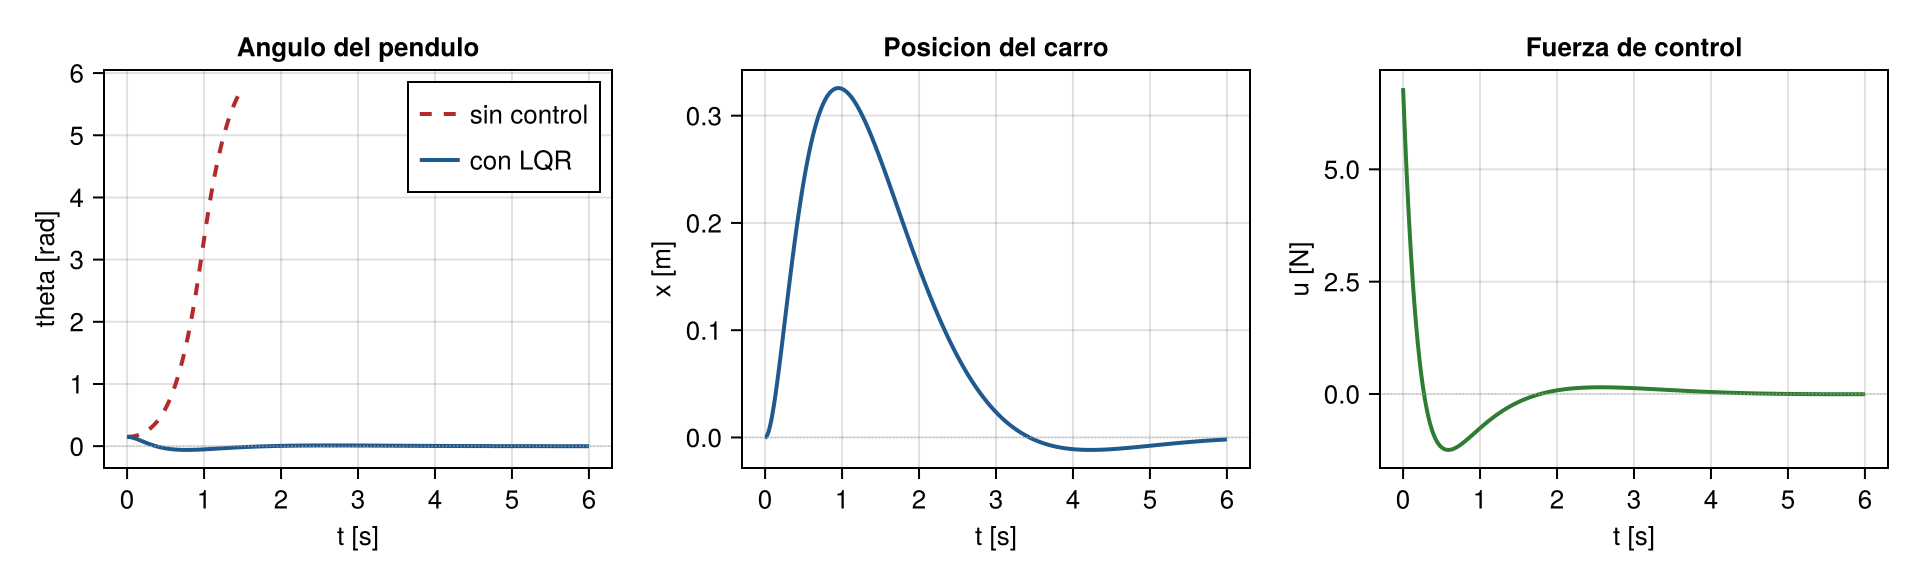
\includegraphics[width=\linewidth]{simple_respuesta.png}
  \caption{Respuesta temporal en lazo cerrado del péndulo simple con la
  ganancia LQR de la \cref{tab:K}, partiendo de una inclinación inicial
  $\theta_0=0.15$~rad. Sin control (rojo, discontinuo) el ángulo diverge; con
  LQR el péndulo vuelve a la vertical en $t_s\approx1.45$~s, con un
  desplazamiento transitorio del carro de $\approx0.33$~m y una fuerza pico de
  $\approx6.8$~N.}
  \label{fig:resp}
\end{figure}

\subsection{Respuesta temporal y comparación de métodos}
\label{sub:resp}

Para verificar los diseños se integró el modelo \emph{no lineal} en lazo
cerrado con la ley $\uv=-K\xv$ mediante un Runge--Kutta explícito
(\texttt{Tsit5}). La \cref{fig:resp} muestra el péndulo simple: sin control el
ángulo crece sin límite en menos de un segundo, mientras que con la ganancia
LQR el sistema regresa al equilibrio en $t_s\approx1.45$~s (umbral
$|\theta|<0.02$~rad $\approx1.1^\circ$), con una fuerza máxima de $6.8$~N, muy por debajo de la saturación de
$\pm50$~N impuesta al actuador.

La \cref{fig:lqr-ack} compara las dos vías de diseño para el simple. El LQR
ubica polos complejos y asienta algo más rápido, con una respuesta levemente
sub-amortiguada; la asignación de polos de Ackermann, al fijar los polos reales
$\{-1,-2,-3,-4\}$, da una respuesta sin oscilación y un esfuerzo de control pico
ligeramente menor. Ambas estabilizan: la diferencia es de criterio de diseño,
no de capacidad.

\begin{figure}[htbp]
  \centering
  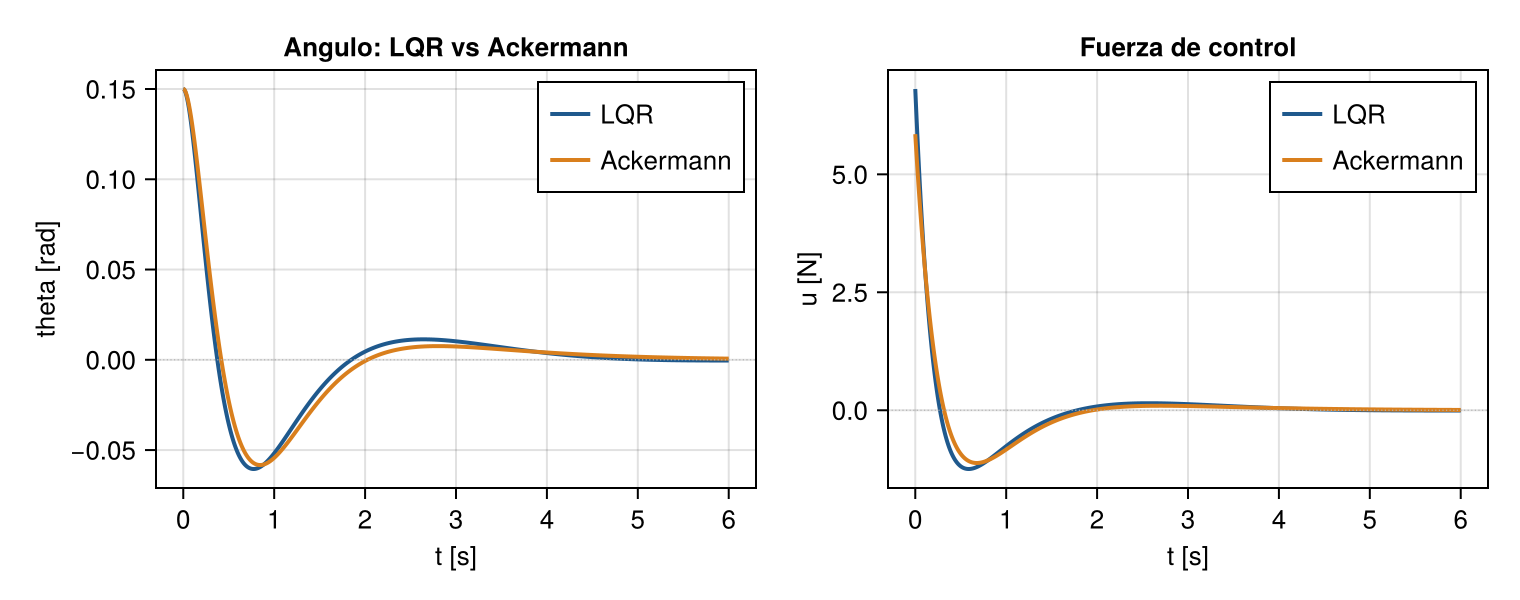
\includegraphics[width=0.86\linewidth]{simple_lqr_vs_acker.png}
  \caption{Péndulo simple: ángulo y esfuerzo de control con LQR frente a
  asignación de polos por Ackermann (polos $\{-1,-2,-3,-4\}$).}
  \label{fig:lqr-ack}
\end{figure}

El péndulo doble (\cref{fig:resp-doble}) confirma que el procedimiento escala
sin cambios conceptuales. Partiendo de $\theta_1=\theta_2=0.1$~rad, sin control
ambos eslabones caen de forma rápida y errática --- el comportamiento típico de
un doble péndulo ---, mientras que el LQR lleva los dos ángulos a cero en
$\approx1.8$~s. Es notable que, pese a que las ganancias del doble son un orden
de magnitud mayores (\cref{tab:K}), para perturbaciones pequeñas la fuerza pico
se mantiene moderada ($4.2$~N); el costo se traslada a una excursión mayor del
carro ($0.43$~m frente a $0.33$~m del simple), que debe maniobrar más para
equilibrar dos eslabones acoplados.

\begin{table}[htbp]
  \centering
  \caption{Métricas de la respuesta en lazo cerrado sobre el modelo no lineal:
  tiempo de asentamiento (umbral $|\theta|<0.02$~rad $\approx1.1^\circ$) y
  fuerza de control pico.}
  \label{tab:metrics}
  \begin{tabular}{@{}lcc@{}}
    \toprule
    \textbf{Caso} & $t_s$ [s] & $\max|u|$ [N]\\
    \midrule
    Simple --- LQR        & 1.45 & 6.8\\
    Simple --- Ackermann  & 1.54 & 5.9\\
    Doble --- LQR         & 1.77 & 4.2\\
    \bottomrule
  \end{tabular}
\end{table}

\begin{figure}[htbp]
  \centering
  
\includegraphics[width=\linewidth]{doble_respuesta.png}
  \caption{Respuesta temporal en lazo cerrado del péndulo doble con la ganancia
  LQR de la \cref{tab:K}, partiendo de $\theta_1=\theta_2=0.1$~rad. Sin control
  (rojo, discontinuo) ambos eslabones caen; con LQR (azul) los dos ángulos se
  estabilizan en $\approx1.8$~s.}
  \label{fig:resp-doble}
\end{figure}

\subsection{Lectura geométrica de las trayectorias}

Con $A_c=A-BK$ diagonalizable, la fórmula \cref{eq:expm-diag} da
\begin{equation}\label{eq:modos}
  e^{A_c t}=\sum_{i=1}^{n} e^{\mu_i t}\,\bm v_i\bm w_i^\top,
\end{equation}
donde $\bm v_i$ y $\bm w_i$ son los eigenvectores derecho e izquierdo
normalizados ($\bm w_i^\top\bm v_j=\delta_{ij}$). Cada sumando es la
proyección de la trayectoria sobre el $i$-ésimo \emph{modo propio} y decae
a la tasa $|\Real(\mu_i)|$. Así, la descomposición espectral de $A_c$
explica la forma con que las trayectorias se aproximan al origen: los
polos más a la izquierda corresponden a los modos que se extinguen más
rápido.

% ============================================================
\section{Conclusiones}
\label{sec:concl}

Se analizaron dos configuraciones del péndulo invertido sobre un carro
--- simple y doble --- con un mismo aparato de álgebra lineal. En ambas,
el formalismo de Euler--Lagrange produjo las ecuaciones de movimiento, y
su linealización por Taylor alrededor del equilibrio inestable dio una
representación en espacio de estados $\dot\xv=A\xv+B\uv$. El
comportamiento del sistema quedó determinado por la exponencial matricial
$e^{At}$ y, a través de ella, por el espectro de $A$: la presencia de
eigenvalores con parte real positiva (uno en el simple, dos en el doble)
es la firma algebraica de la inestabilidad, y su cálculo se apoyó en el
polinomio característico y en la diagonalización justificada por la teoría
del polinomio minimal.

El criterio de rango de Kalman estableció la controlabilidad y
observabilidad completas de las dos configuraciones, y el teorema de
asignación de polos garantizó que el espectro de $A-BK$ puede colocarse
por realimentación de estado. Se diseñaron controladores estabilizantes
por asignación de polos (Ackermann) y por regulación óptima (LQR, vía la
ecuación de Riccati), verificados sobre el modelo no lineal. El péndulo
doble mostró que el procedimiento escala sin cambios conceptuales, solo a
costa de matrices mayores y mayor esfuerzo de control.

La verificación por simulación cerró el ciclo: integrando el modelo
\emph{no lineal} en lazo cerrado, los controladores llevaron ambas
configuraciones a una vecindad de la vertical ($|\theta|<0.02$~rad) en menos de
dos segundos (\cref{tab:metrics}), lo
que confirma que el diseño basado en el modelo \emph{linealizado} es válido en
la vecindad del punto de operación. Toda la cadena --- modelado, linealización,
análisis y control --- se implementó y ejecutó en Julia, y reproduce
numéricamente los valores reportados (\cref{anx:impl}).

En conjunto, el trabajo evidencia que un puñado de conceptos del álgebra
lineal --- exponencial matricial, análisis espectral, teorema de
Cayley--Hamilton, descomposiciones canónicas, teoría del rango y
subespacios invariantes --- constituye el lenguaje natural para modelar,
analizar y controlar un sistema dinámico.

% ============================================================
\appendix
\renewcommand{\thesection}{\Alph{section}}

\section{Derivación de los lagrangianos}
\label{anx:lag}

\paragraph{Péndulo simple.} Con \cref{eq:T-simple,eq:V-simple} y
$L=T-V$, las derivadas parciales para $q_1=x$ son
$\partial L/\partial\dot x=(M{+}m)\dot x+mL\dot\theta\cos\theta$ y
$\partial L/\partial x=0$; para $q_2=\theta$,
$\partial L/\partial\dot\theta=(I{+}mL^2)\dot\theta+mL\dot x\cos\theta$ y
$\partial L/\partial\theta=-mL\dot x\dot\theta\sin\theta+mgL\sin\theta$.
Sustituyendo en \cref{eq:EL} con $Q_1=u-b\dot x$, $Q_2=0$, se obtienen
\cref{eq:nl-simple}. Linealizando con \cref{eq:smallangle} el sistema
$2\times2$
\begin{equation*}
\begin{pmatrix}M{+}m & mL\\ mL & I{+}mL^2\end{pmatrix}
\begin{pmatrix}\ddot x\\\ddot\theta\end{pmatrix}=
\begin{pmatrix}u-b\dot x\\ mgL\,\theta\end{pmatrix},
\end{equation*}
de determinante $D_0=(M{+}m)(I{+}mL^2)-(mL)^2$, e invirtiendo la matriz de
masa se llega directamente a \cref{eq:AB-simple}.

\paragraph{Péndulo doble.} Con las posiciones $\rv_1,\rv_2$ de la
\cref{sub:doble} y $L=T-V$, la aplicación de \cref{eq:EL} a las tres
coordenadas produce \cref{eq:nl-doble} con la matriz de masa
$\mathbf{M}(q)$ de \cref{eq:Mq} y el vector de gravedad $\mathbf{G}(q)$ de
\cref{eq:Gq}. Evaluando $\mathbf{M}(q)$ en $\theta_1=\theta_2=0$
($c_1=c_2=c_{12}=1$) y linealizando $\mathbf{G}(q)$ con
\cref{eq:smallangle} se obtienen \cref{eq:A-doble,eq:B-doble}. Haciendo
$m_2=0$ se recupera el caso simple, lo que verifica la derivación.

\section{Verificación numérica}
\label{anx:num}

Para el péndulo simple, con $D_0=0.1075$, las matrices numéricas son
\begin{equation*}
A=\begin{pmatrix}
0&1&0&0\\0&-0.093&-2.053&0\\0&0&0&1\\0&0.140&17.795&0
\end{pmatrix},\quad
B=\begin{pmatrix}0\\0.930\\0\\-1.395\end{pmatrix},
\end{equation*}
con espectro $\sigma(A)=\{+4.21,\ 0,\ -0.077,\ -4.23\}$ y
$\rank(\calC)=\rank(\calO)=4$. Los cuatro eigenvalores son distintos, de
modo que $A$ es diagonalizable (\cref{cor:jordan}). Para el péndulo doble,
$\sigma(A)=\{\pm8.57,\ \pm4.09,\ 0,\ 0\}$ y
$\rank(\calC)=\rank(\calO)=6$. Las ganancias $K$ y los espectros en lazo
cerrado son los consignados en la \cref{tab:K}.

% ============================================================
\section{Implementación: organización del código y flujo de archivos}
\label{anx:impl}

El proyecto se implementó en Julia y se ejecuta de principio a fin: todos los
valores de las \cref{tab:abierto,tab:K} y las figuras de la \cref{sec:result}
se generan corriendo los scripts descritos aquí. El diseño separa
deliberadamente la \emph{física} (distinta en cada configuración) de los
\emph{algoritmos de álgebra lineal} (idénticos), de modo que el péndulo doble
reutiliza sin cambios el análisis y el control programados para el simple.

\subsection*{Flujo de archivos}

\begin{lstlisting}[language={},keywordstyle=]
Proyecto/
  main_simple.jl        Pipeline del pendulo simple (Configuracion I)
  main_double.jl        Pipeline del pendulo doble  (Configuracion II)
  setup.jl              Instalacion de dependencias
  Project.toml          Entorno unico de todo el proyecto
  src/
    model_simple.jl     Simple: parametros y EOM no lineales (Euler-Lagrange)
    model_double.jl     Doble:  parametros y EOM no lineales
    linearization.jl    Linealizacion (A,B,C,D), espectro y matrices de Kalman
    controller.jl       LQR (Riccati via Hamiltoniano) y Ackermann (genericos)
    animation_simple.jl Animacion del simple
    animation_double.jl Animacion del doble
  notebooks/
    01_exploracion_simple.jl   Explorador interactivo (Pluto) del simple
    02_exploracion_doble.jl    Explorador interactivo (Pluto) del doble
  figures/              Graficas y animaciones generadas
  resumen_tecnico/      Este informe (LaTeX) y make_report_figs.jl
\end{lstlisting}

El flujo de datos en cada \texttt{main\_*.jl} reproduce el orden lógico del
informe: \texttt{model} entrega el campo no lineal $f(\xv,u)$;
\texttt{linearization} produce $(A,B,C,D)$ junto con el análisis espectral y de
Kalman; \texttt{controller} calcula la ganancia $K$; y la simulación no lineal
en lazo cerrado cierra la verificación. Las rutinas de \texttt{controller} y el
análisis de \texttt{linearization} son \emph{genéricos en la dimensión del
estado}, por lo que operan igual sobre el sistema $4\times4$ del simple y el
$6\times6$ del doble.

\subsection*{Extractos representativos}

La solución de la ecuación de Riccati (\cref{obs:hamilton}) se traduce
directamente en código: se arma la matriz hamiltoniana $H$, se toman sus $n$
eigenvectores estables y se forma $P=V_2V_1^{-1}$.

\begin{lstlisting}
function solve_care(A, B, Q, R)
    n = size(A, 1)
    S = B * inv(R) * B'
    H = [A -S; -Q -A']                        # matriz hamiltoniana 2n x 2n
    eig = eigen(H)
    stable = findall(real.(eig.values) .< 0)  # subespacio invariante estable
    V = eig.vectors[:, stable]
    V1 = V[1:n, :]; V2 = V[n+1:2n, :]
    P = real.(V2 / V1)                         # P = V2 * inv(V1)
    return (P + P') / 2                         # simetrizar
end
\end{lstlisting}

El Jacobiano analítico del péndulo doble (\cref{eq:A-doble}) se escribe entrada
por entrada; coincide con el Jacobiano numérico de las ecuaciones no lineales
hasta $10^{-11}$, lo que valida ambos cálculos.

\begin{lstlisting}
A = zeros(6, 6)
A[1, 2] = 1.0
A[2, 3] = -g * (m1 + m2) / M
A[3, 4] = 1.0
A[4, 3] = g * (M + m1) * (m1 + m2) / (M * L1 * m1)
A[4, 5] = -g * m2 / (L1 * m1)
A[5, 6] = 1.0
A[6, 3] = -g * (m1 + m2) / (L2 * m1)
A[6, 5] = g * (m1 + m2) / (L2 * m1)
\end{lstlisting}

Las ecuaciones no lineales del doble se obtienen armando la matriz de masa
$\mathbf{M}(q)$ (\cref{eq:Mq}) y el lado derecho, y despejando las aceleraciones
al resolver el sistema lineal $\mathbf{M}(q)\,\ddot q=\text{rhs}$.

\begin{lstlisting}
Mq = [ M+m1+m2          (m1+m2)*L1*c1     m2*L2*c2;
       (m1+m2)*L1*c1    (m1+m2)*L1^2      m2*L1*L2*c12;
       m2*L2*c2         m2*L1*L2*c12      m2*L2^2 ]
rhs = [ F + (m1+m2)*L1*s1*w1^2 + m2*L2*s2*w2^2,
        (m1+m2)*g*L1*s1 - m2*L1*L2*s12*w2^2,
        m2*g*L2*s2 + m2*L1*L2*s12*w1^2 ]
qdd = Mq \ rhs        # aceleraciones [ddx, ddtheta1, ddtheta2]
\end{lstlisting}

\subsection*{Estado actual del proyecto}

Ambas configuraciones están implementadas, ejecutadas y verificadas en Julia.
Los scripts \texttt{main\_simple.jl} y \texttt{main\_double.jl} reproducen los
eigenvalores de lazo abierto y cerrado, los rangos de Kalman y las ganancias de
las \cref{tab:abierto,tab:K}, y generan las figuras de la \cref{sec:result}. Se
incluyen además dos cuadernos interactivos en Pluto (carpeta
\texttt{notebooks/}) que permiten variar los parámetros físicos y los pesos del
controlador con deslizadores, recalculando todo el análisis en vivo. El script
\texttt{make\_report\_figs.jl} regenera las figuras de respuesta temporal de
este informe.

% ============================================================
\begin{thebibliography}{9}

\bibitem{ogata2010}
K.~Ogata, \emph{Modern Control Engineering}, 5.\textsuperscript{a} ed.
Upper Saddle River, NJ: Prentice Hall, 2010.

\bibitem{chen1999}
C.-T.~Chen, \emph{Linear System Theory and Design}, 3.\textsuperscript{a} ed.
New York: Oxford University Press, 1999.

\bibitem{hoffman1971}
K.~Hoffman y R.~Kunze, \emph{Linear Algebra}, 2.\textsuperscript{a} ed.
Englewood Cliffs, NJ: Prentice Hall, 1971.

\bibitem{strang2016}
G.~Strang, \emph{Introduction to Linear Algebra}, 5.\textsuperscript{a} ed.
Wellesley, MA: Wellesley--Cambridge Press, 2016.

\bibitem{hirsch2004}
M.~W.~Hirsch, S.~Smale y R.~L.~Devaney, \emph{Differential Equations,
Dynamical Systems, and an Introduction to Chaos}, 2.\textsuperscript{a} ed.
San Diego: Elsevier Academic Press, 2004.

\bibitem{golub2013}
G.~H.~Golub y C.~F.~Van Loan, \emph{Matrix Computations},
4.\textsuperscript{a} ed. Baltimore: Johns Hopkins University Press, 2013.

\bibitem{notas2026}
A.~Vélez, \emph{Notas del curso: Cálculo de Variaciones}. Universidad Nacional de Colombia, Sede Medellín, 2026.

\end{thebibliography}

\end{document}